\chapter{Time complexity}

\index{time complexity}

The efficiency of algorithms is important in competitive programming.
Usually, it is easy to design an algorithm
that solves the problem slowly,
but the real challenge is to invent a
fast algorithm.
If an algorithm is too slow, it will get only
partial points or no points at all.

The \key{time complexity} of an algorithm
estimates how much time the algorithm will use
for some input.
The idea is to represent the efficiency
as an function whose parameter is the size of the input.
By calculating the time complexity,
we can estimate if the algorithm is good enough
without implementing it.

\section{Calculation rules}

The time complexity of an algorithm
is denoted $O(\cdots)$
where the three dots represent some
function.
Usually, the variable $n$ denotes
the input size.
For example, if the input is an array of numbers,
$n$ will be the size of the array,
and if the input is a string,
$n$ will be the length of the string.

\subsubsection*{Loops}

The typical reason why an algorithm is slow is
that it contains many loops that go through the input.
The more nested loops the algorithm contains,
the slower it is.
If there are $k$ nested loops,
the time complexity is $O(n^k)$.

For example, the time complexity of the following code is $O(n)$:
\begin{lstlisting}
for (int i = 1; i <= n; i++) {
    // code
}
\end{lstlisting}

Correspondingly, the time complexity of the following code is $O(n^2)$:
\begin{lstlisting}
for (int i = 1; i <= n; i++) {
    for (int j = 1; j <= n; j++) {
        // code
    }
}
\end{lstlisting}

\subsubsection*{Order of magnitude}

A time complexity doesn't tell the exact number
of times the code inside a loop is executed,
but it only tells the order of magnitude.
In the following examples, the code inside the loop
is executed $3n$, $n+5$ and $\lceil n/2 \rceil$ times,
but the time complexity of each code is $O(n)$.

\begin{lstlisting}
for (int i = 1; i <= 3*n; i++) {
    // code
}
\end{lstlisting}

\begin{lstlisting}
for (int i = 1; i <= n+5; i++) {
    // code
}
\end{lstlisting}

\begin{lstlisting}
for (int i = 1; i <= n; i += 2) {
    // code
}
\end{lstlisting}

As another example,
the time complexity of the following code is $O(n^2)$:

\begin{lstlisting}
for (int i = 1; i <= n; i++) {
    for (int j = i+1; j <= n; j++) {
        // code
    }
}
\end{lstlisting}

\subsubsection*{Phases}

If the code consists of consecutive phases,
the total time complexity is the largest
time complexity of a single phase.
The reason for this is that the slowest
phase is usually the bottleneck of the code
and the other phases are not important.

For example, the following code consists
of three phases with time complexities
$O(n)$, $O(n^2)$ and $O(n)$.
Thus, the total time complexity is $O(n^2)$.

\begin{lstlisting}
for (int i = 1; i <= n; i++) {
    // code
}
for (int i = 1; i <= n; i++) {
    for (int j = 1; j <= n; j++) {
        // code
    }
}
for (int i = 1; i <= n; i++) {
    // code
}
\end{lstlisting}

\subsubsection*{Several variables}

Sometimes the time complexity depends on
several variables.
In this case, the formula for the time complexity
contains several variables.

For example, the time complexity of the
following code is $O(nm)$:

\begin{lstlisting}
for (int i = 1; i <= n; i++) {
    for (int j = 1; j <= m; j++) {
        // code
    }
}
\end{lstlisting}

\subsubsection*{Recursion}

The time complexity of a recursive function
depends on the number of times the function is called
and the time complexity of a single call.
The total time complexity is the product of
these values.

For example, consider the following function:
\begin{lstlisting}
void f(int n) {
    if (n == 1) return;
    f(n-1);
}
\end{lstlisting}
The call $\texttt{f}(n)$ causes $n$ function calls,
and the time complexity of each call is $O(1)$.
Thus, the total time complexity is $O(n)$.

As another example, consider the following function:
\begin{lstlisting}
void g(int n) {
    if (n == 1) return;
    g(n-1);
    g(n-1);
}
\end{lstlisting}
In this case the function branches into two parts.
Thus, the call $\texttt{g}(n)$ causes the following calls:
\begin{center}
\begin{tabular}{rr}
call & amount \\
\hline
$\texttt{g}(n)$ & 1 \\
$\texttt{g}(n-1)$ & 2 \\
$\cdots$ & $\cdots$ \\
$\texttt{g}(1)$ & $2^{n-1}$ \\
\end{tabular}
\end{center}
Based on this, the time complexity is
\[1+2+4+\cdots+2^{n-1} = 2^n-1 = O(2^n).\]

\section{Complexity classes}

\index{complexity classes}

Typical complexity classes are:

\begin{description}
\item[$O(1)$]
\index{constant-time algorithm}
The running time of a \key{constant-time} algorithm
doesn't depend on the input size.
A typical constant-time algorithm is a direct
formula that calculates the answer.

\item[$O(\log n)$]
\index{logarithmic algorithm}
A \key{logarithmic} algorithm often halves
the input size at each step.
The reason for this is that the logarithm
$\log_2 n$ equals the number of times
$n$ must be divided by 2 to produce 1.

\item[$O(\sqrt n)$]
The running time of this kind of algorithm
is between $O(\log n)$ and $O(n)$.
A special feature of the square root is that
$\sqrt n = n/\sqrt n$, so the square root lies
''in the middle'' of the input.

\item[$O(n)$]
\index{linear algorithm}
A \key{linear} algorithm goes through the input
a constant number of times.
This is often the best possible time complexity
because it is usually needed to access each
input element at least once before
reporting the answer.

\item[$O(n \log n)$]
This time complexity often means that the
algorithm sorts the input
because the time complexity of efficient
sorting algorithms is $O(n \log n)$.
Another possibility is that the algorithm
uses a data structure where the time
complexity of each operation is $O(\log n)$.

\item[$O(n^2)$]
\index{quadratic algorithm}
A \key{quadratic} algorithm often contains
two nested loops.
It is possible to go through all pairs of
input elements in $O(n^2)$ time.

\item[$O(n^3)$]
\index{cubic algorithm}
A \key{cubic} algorithm often contains
three nested loops.
It is possible to go through all triplets of
input elements in $O(n^3)$ time.

\item[$O(2^n)$]
This time complexity often means that
the algorithm iterates through all
subsets of the input elements.
For example, the subsets of $\{1,2,3\}$ are
$\emptyset$, $\{1\}$, $\{2\}$, $\{3\}$, $\{1,2\}$,
$\{1,3\}$, $\{2,3\}$ and $\{1,2,3\}$.

\item[$O(n!)$]
This time complexity often means that
the algorithm iterates trough all
permutations of the input elements.
For example, the permutations of $\{1,2,3\}$ are
$(1,2,3)$, $(1,3,2)$, $(2,1,3)$, $(2,3,1)$,
$(3,1,2)$ and $(3,2,1)$.

\end{description}

\index{polynomial algorithm}
An algorithm is \key{polynomial}
if its time complexity is at most $O(n^k)$
where $k$ is a constant.
All the above time complexities except
$O(2^n)$ and $O(n!)$ are polynomial.
In practice, the constant $k$ is usually small,
and therefore a polynomial time complexity
means that the algorithm is \emph{efficient}.

\index{NP-hard problem}

Most algorithms in this book are polynomial.
Still, there are many important problems for which
no polynomial algorithm is known, i.e.,
nobody knows how to solve the problem efficiently.
\key{NP-hard} problems are an important set
of problems for which no polynomial algorithm is known.

\section{Tehokkuuden arviointi}

Aikavaativuuden hyötynä on,
että sen avulla voi arvioida ennen algoritmin
toteuttamista, onko algoritmi riittävän nopea
tehtävän ratkaisemiseen.
Lähtökohtana arviossa on, että nykyaikainen tietokone
pystyy suorittamaan sekunnissa joitakin
satoja miljoonia koodissa olevia komentoja.

Oletetaan esimerkiksi, että tehtävän aikaraja on 
yksi sekunti ja syötteen koko on $n=10^5$.
Jos algoritmin aikavaativuus on $O(n^2)$,
algoritmi suorittaa noin $(10^5)^2=10^{10}$ komentoa.
Tähän kuluu aikaa arviolta kymmeniä sekunteja,
joten algoritmi vaikuttaa liian hitaalta tehtävän ratkaisemiseen.

Käänteisesti syötteen koosta voi päätellä,
kuinka tehokasta algoritmia tehtävän laatija odottaa
ratkaisijalta.
Seuraavassa taulukossa on joitakin hyödyllisiä arvioita,
jotka olettavat, että tehtävän aikaraja on yksi sekunti.

\begin{center}
\begin{tabular}{ll}
syötteen koko ($n$) & haluttu aikavaativuus \\
\hline
$n \le 10^{18}$ & $O(1)$ tai $O(\log n)$ \\
$n \le 10^{12}$ & $O(\sqrt n)$ \\
$n \le 10^6$ & $O(n)$ tai $O(n \log n)$ \\
$n \le 5000$ & $O(n^2)$ \\
$n \le 500$ & $O(n^3)$ \\
$n \le 25$ & $O(2^n)$ \\
$n \le 10$ & $O(n!)$ \\
\end{tabular}
\end{center}

Esimerkiksi jos syötteen koko on $n=10^5$,
tehtävän laatija odottaa luultavasti
algoritmia, jonka aikavaativuus on $O(n)$ tai $O(n \log n)$.
Tämä tieto helpottaa algoritmin suunnittelua,
koska se rajaa pois monia lähestymistapoja,
joiden tuloksena olisi hitaampi aikavaativuus.

\index{vakiokerroin}

Aikavaativuus ei kerro kuitenkaan kaikkea algoritmin
tehokkuudesta, koska se kätkee toteutuksessa olevat
\key{vakiokertoimet}. Esimerkiksi aikavaativuuden $O(n)$
algoritmi voi tehdä käytännössä $n/2$ tai $5n$ operaatiota.
Tällä on merkittävä vaikutus algoritmin
todelliseen ajankäyttöön.

\section{Suurin alitaulukon summa}

\index{suurin alitaulukon summa@suurin alitaulukon summa}

Usein ohjelmointitehtävän ratkaisuun on monta
luontevaa algoritmia, joiden aikavaativuudet eroavat.
Tutustumme seuraavaksi klassiseen ongelmaan,
jonka suoraviivaisen ratkaisun aikavaativuus on $O(n^3)$,
mutta algoritmia parantamalla aikavaativuudeksi
tulee ensin $O(n^2)$ ja lopulta $O(n)$.

Annettuna on taulukko, jossa on $n$ kokonaislukua
$x_1,x_2,\ldots,x_n$, ja tehtävänä on etsiä
taulukon \key{suurin alitaulukon summa}
eli mahdollisimman suuri summa
taulukon yhtenäisellä välillä.
Tehtävän kiinnostavuus on siinä, että taulukossa
saattaa olla negatiivisia lukuja.
Esimerkiksi taulukossa
\begin{center}
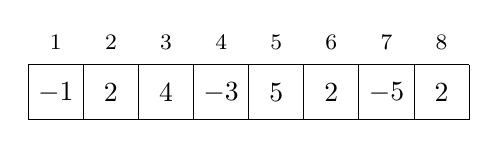
\begin{tikzpicture}[scale=0.7]
\draw (0,0) grid (8,1);

\node at (0.5,0.5) {$-1$};
\node at (1.5,0.5) {$2$};
\node at (2.5,0.5) {$4$};
\node at (3.5,0.5) {$-3$};
\node at (4.5,0.5) {$5$};
\node at (5.5,0.5) {$2$};
\node at (6.5,0.5) {$-5$};
\node at (7.5,0.5) {$2$};

\footnotesize
\node at (0.5,1.4) {$1$};
\node at (1.5,1.4) {$2$};
\node at (2.5,1.4) {$3$};
\node at (3.5,1.4) {$4$};
\node at (4.5,1.4) {$5$};
\node at (5.5,1.4) {$6$};
\node at (6.5,1.4) {$7$};
\node at (7.5,1.4) {$8$};
\end{tikzpicture}
\end{center}
\begin{samepage}
suurimman summan $10$ tuottaa seuraava alitaulukko:
\begin{center}
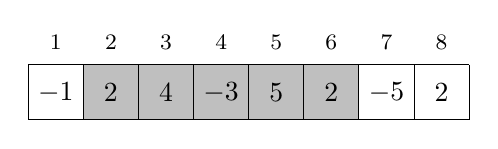
\begin{tikzpicture}[scale=0.7]
\fill[color=lightgray] (1,0) rectangle (6,1);
\draw (0,0) grid (8,1);

\node at (0.5,0.5) {$-1$};
\node at (1.5,0.5) {$2$};
\node at (2.5,0.5) {$4$};
\node at (3.5,0.5) {$-3$};
\node at (4.5,0.5) {$5$};
\node at (5.5,0.5) {$2$};
\node at (6.5,0.5) {$-5$};
\node at (7.5,0.5) {$2$};

\footnotesize
\node at (0.5,1.4) {$1$};
\node at (1.5,1.4) {$2$};
\node at (2.5,1.4) {$3$};
\node at (3.5,1.4) {$4$};
\node at (4.5,1.4) {$5$};
\node at (5.5,1.4) {$6$};
\node at (6.5,1.4) {$7$};
\node at (7.5,1.4) {$8$};
\end{tikzpicture}
\end{center}
\end{samepage}


\subsubsection{Ratkaisu 1}

Suoraviivainen ratkaisu tehtävään on käydä
läpi kaikki tavat valita alitaulukko taulukosta,
laskea jokaisesta vaihtoehdosta lukujen summa
ja pitää muistissa suurinta summaa.
Seuraava koodi toteuttaa tämän algoritmin:

\begin{lstlisting}
int p = 0;
for (int a = 1; a <= n; a++) {
    for (int b = a; b <= n; b++) {
        int s = 0;
        for (int c = a; c <= b; c++) {
            s += x[c];
        }
        p = max(p,s);
    }
}
cout << p << "\n";
\end{lstlisting}

Koodi olettaa, että luvut on tallennettu taulukkoon \texttt{x},
jota indeksoidaan $1 \ldots n$.
Muuttujat $a$ ja $b$ valitsevat alitaulukon ensimmäisen
ja viimeisen luvun, ja alitaulukon summa lasketaan muuttujaan $s$.
Muuttujassa $p$ on puolestaan paras haun aikana löydetty summa.

Algoritmin aikavaativuus on $O(n^3)$, koska siinä on kolme
sisäkkäistä silmukkaa ja jokainen silmukka käy läpi $O(n)$ lukua.

\subsubsection{Ratkaisu 2}

Äskeistä ratkaisua on helppoa tehostaa hankkiutumalla
eroon sisimmästä silmukasta.
Tämä on mahdollista laskemalla summaa samalla,
kun alitaulukon oikea reuna liikkuu eteenpäin.
Tuloksena on seuraava koodi:

\begin{lstlisting}
int p = 0;
for (int a = 1; a <= n; a++) {
    int s = 0;
    for (int b = a; b <= n; b++) {
        s += x[b];
        p = max(p,s);
    }
}
cout << p << "\n";
\end{lstlisting}
Tämän muutoksen jälkeen koodin aikavaativuus on $O(n^2)$.

\subsubsection{Ratkaisu 3}

Yllättävää kyllä, tehtävään on olemassa myös
$O(n)$-aikainen ratkaisu eli koodista pystyy
karsimaan vielä yhden silmukan.
Ideana on laskea taulukon jokaiseen
kohtaan, mikä on suurin alitaulukon
summa, jos alitaulukko päättyy kyseiseen kohtaan.
Tämän jälkeen ratkaisu tehtävään on suurin
näistä summista.

Tarkastellaan suurimman summan tuottavan
alitaulukon etsimistä,
kun valittuna on alitaulukon loppukohta $k$.
Vaihtoehtoja on kaksi:
\begin{enumerate}
\item Alitaulukossa on vain kohdassa $k$ oleva luku.
\item Alitaulukossa on ensin jokin kohtaan $k-1$ päättyvä alitaulukko
ja sen jälkeen kohdassa $k$ oleva luku.
\end{enumerate}

Koska tavoitteena on löytää alitaulukko,
jonka lukujen summa on suurin,
tapauksessa 2 myös kohtaan $k-1$ päättyvän
alitaulukon tulee olla sellainen,
että sen summa on suurin.
Niinpä tehokas ratkaisu syntyy käymällä läpi
kaikki alitaulukon loppukohdat järjestyksessä
ja laskemalla jokaiseen kohtaan suurin
mahdollinen kyseiseen kohtaan päättyvän alitaulukon summa.

Seuraava koodi toteuttaa ratkaisun:

\begin{lstlisting}
int p = 0, s = 0;
for (int k = 1; k <= n; k++) {
    s = max(x[k],s+x[k]);
    p = max(p,s);
}
cout << p << "\n";
\end{lstlisting}

Algoritmissa on vain yksi silmukka,
joka käy läpi taulukon luvut,
joten sen aikavaativuus on $O(n)$.
Tämä on myös paras mahdollinen aikavaativuus,
koska minkä tahansa algoritmin täytyy käydä
läpi ainakin kerran taulukon sisältö.

\subsubsection{Tehokkuusvertailu}

On kiinnostavaa tutkia, kuinka tehokkaita algoritmit
ovat käytännössä.
Seuraava taulukko näyttää, kuinka nopeasti äskeiset
ratkaisut toimivat eri $n$:n arvoilla
nykyaikaisella tietokoneella.

Jokaisessa testissä syöte on muodostettu satunnaisesti.
Ajankäyttöön ei ole laskettu syötteen lukemiseen
kuluvaa aikaa.

\begin{center}
\begin{tabular}{rrrr}
taulukon koko $n$ & ratkaisu 1 & ratkaisu 2 & ratkaisu 3 \\
\hline
$10^2$ & $0{,}0$ s & $0{,}0$ s & $0{,}0$ s \\
$10^3$ & $0{,}1$ s & $0{,}0$ s & $0{,}0$ s \\
$10^4$ & > $10,0$ s & $0{,}1$ s & $0{,}0$ s \\
$10^5$ & > $10,0$ s & $5{,}3$ s & $0{,}0$ s \\
$10^6$ & > $10,0$ s & > $10,0$ s & $0{,}0$ s \\
$10^7$ & > $10,0$ s & > $10,0$ s & $0{,}0$ s \\
\end{tabular}
\end{center}

Vertailu osoittaa,
että pienillä syötteillä kaikki algoritmit
ovat tehokkaita,
mutta suuremmat syötteet tuovat esille
merkittäviä eroja algoritmien suoritusajassa.
$O(n^3)$-aikainen ratkaisu 1 alkaa hidastua,
kun $n=10^3$, ja $O(n^2)$-aikainen ratkaisu 2
alkaa hidastua, kun $n=10^4$.
Vain $O(n)$-aikainen ratkaisu 3 selvittää
suurimmatkin syötteet salamannopeasti.
